\begin{tikzpicture}
    \node at (0,0) 
    {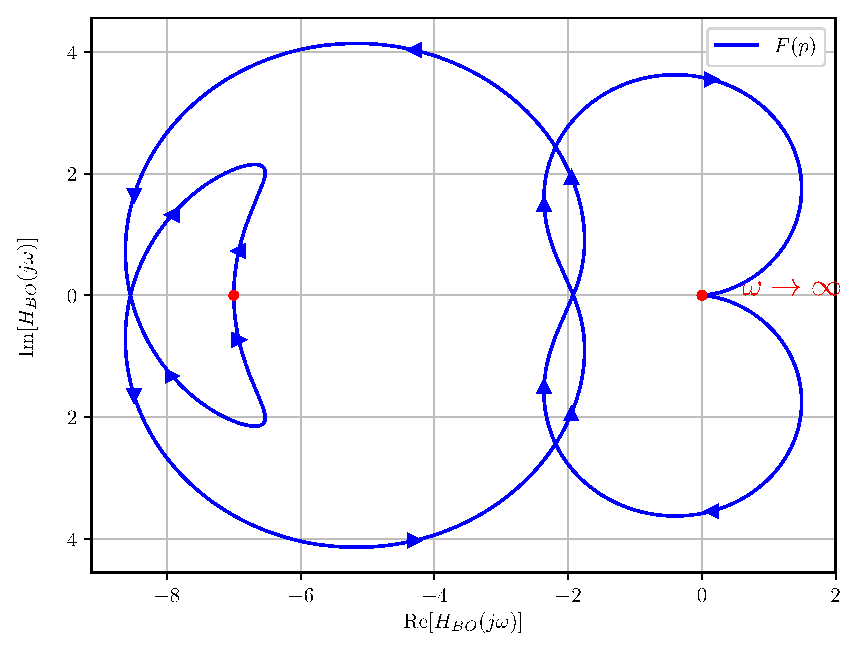
\includegraphics
    [width=0.8\textwidth]{fig/chap_stab/exercice_nyquist_chap_stab_ex1_enonce.eps}};
    \node at (-1.75,0.5) {\large\textcolor{col3}{$\boldsymbol{N=2}$}};
    \pgfmathsetmacro{\vx}{0.9563}
    \pgfmathsetmacro{\vy}{0.2923}
    \pgfmathsetmacro{\rr}{1.35}
    \pgfmathsetmacro{\a}{-3.75}
    \pgfmathsetmacro{\b}{1.5}
    \draw[ultra thick,col3] (\a,\b) --+ (\rr*\vx,\rr*\vy);
    \pgfmathsetmacro{\rr}{1.52}
    \pgfmathsetmacro{\a}{-4.05}
    \pgfmathsetmacro{\b}{1.0}
    \draw[ultra thick,col3] (\a,\b) --+ (\rr*\vx,\rr*\vy);
    \pgfmathsetmacro{\rr}{1.6}
    \pgfmathsetmacro{\a}{-4.25}
    \pgfmathsetmacro{\b}{0.5}
    \draw[ultra thick,col3] (\a,\b) --+ (\rr*\vx,\rr*\vy);
    \pgfmathsetmacro{\rr}{1.4}
    \pgfmathsetmacro{\a}{-4.15}
    \pgfmathsetmacro{\b}{0.0}
    \draw[ultra thick,col3] (\a,\b) --+ (\rr*\vx,\rr*\vy);
    \pgfmathsetmacro{\rr}{1.2}
    \pgfmathsetmacro{\a}{-3.9}
    \pgfmathsetmacro{\b}{-0.5}
    \draw[ultra thick,col3] (\a,\b) --+ (\rr*\vx,\rr*\vy);
    \pgfmathsetmacro{\rr}{0.85}
    \pgfmathsetmacro{\a}{-3.35}
    \pgfmathsetmacro{\b}{-1.0}
    \draw[ultra thick,col3] (\a,\b) --+ (\rr*\vx,\rr*\vy);
\end{tikzpicture}
